


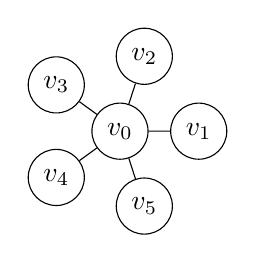
\begin{tikzpicture}
\tikzstyle{every node}=[draw,shape=circle];
\node (v0) at (0:0) {$v_0$};
\node (v1) at ( 0:1) {$v_1$};
\node (v2) at ( 72:1) {$v_2$};
\node (v3) at (2*72:1) {$v_3$};
\node (v4) at (3*72:1) {$v_4$};
\node (v5) at (4*72:1) {$v_5$};
\draw (v0) -- (v1)
(v0) -- (v2)
(v0) -- (v3)
(v0) -- (v4)
(v0) -- (v5);
\end{tikzpicture}

